\chapter{Swarm Simulation Software}
\label{ch:SwarmSimulationSoftware}

This chapter describes the framework and implementation of \SWEEP{}, the \SWEEPexp{}.  The implementation of \SWEEP{} discussed in this chapter is an extension of the original \SWEEP{} implementation created by Palmer and Hantak~\cite{hantak:SWEEP}. 

\section{Existing Swarm Simulation Software}

Aside from \SWEEP, there are a number of existing swarm simulation packages that are currently available.
Perhaps the best known is \textsc{Swarm}.\footnote{\url{http://www.swarm.org}}  \textsc{Swarm}, originally developed at the Santa Fe Institute, provides an extensive library of software components designed for multi-agent simulations of complex systems.
\textsc{Breve}\footnote{\url{http://www.spiderland.org/breve}} is a 3-D simulation environment designed for multi-agent simulations and artificial life research .  \textsc{Breve} includes an OpenGL display engine that allows a user to explore simulated worlds from different angles and also provides the ability to create movies from simulations.  
Finally, \textsc{RePast}\footnote{\url{http://repast.sourceforge.net}} (\qw{Recursive Porous Agent Simulation Toolkit}) is an agent-based simulation toolkit designed specifically for social science applications.  \textsc{RePast} permits the systematic study of complex system behaviors through controlled and replicable computational experiments.  \textsc{RePast} has an extensive set of libraries relating to topics such as networking, statistics, and modeling.  Another feature of \textsc{RePast} is the built-in adaptive tools, such as a genetic algorithm package, that allow a simulation to tune itself.  A more comprehensive comparison of available swarm/multi-agent software packages was performed in \cite{rtobias:SwarmSoftware}.

In terms of functionality, each of these simulation packages, including \SWEEP, contain similar abilities.  Each is implemented in a cross-platform manner, provides the user with an extendable architecture, and is not limited to any one type of simulation.  Where \SWEEP differs from \textsc{Swarm}, \textsc{Breve}, and \textsc{RePast} is in that \SWEEP attempts to separate the programming required for modeling from the development of the simulation itself.  Thus for example, the initial implementation of a new agent will require the development of Java code, but the usage of that agent will not require any programming.  In the current implementation of \SWEEP, this goal is realized through the XML simulation specification file that allows a user to build complex simulations without the need to write Java code.

\section{Design Overview}

\SWEEP{} identifies four major software components for a swarm simulation: \jclass{Simulation}, \jclass{Agent}, \jclass{Environment}, and \jclass{Probe}.  A \jclass{Simulation} object is composed of at least one \jclass{Agent} object, one or more \jclass{Environment} objects, and zero or more \jclass{Probe} objects. A \jclass{Simulation} object is responsible for constructing the various simulation components, establishing the manner in which the simulation components communicate and interact, and managing the runtime aspects of the simulation.  Associated with a \jclass{Simulation} is one or more \jclass{Agents}.  An \jclass{Agent} represents a logical individual within a simulation, which in implementation can in fact be a collection (\qw{swarm}) of other \jclass{Agents}. The \jclass{Environment} components associated with a \jclass{Simulation} define the space where \jclass{Agents} exist, providing a context for the sensing and actuation.  Finally, \jclass{Probes} define methods of extracting internal simulation data from, and inserting external information into, a running simulation.

The overall design goal for \SWEEP{} was the creation of a flexible, general-purpose swarm algorithm testing and development platform targeted for both users and developers alike. The high-level overview of the \SWEEP{} design can be seen in \refFigure{SweepDiagram}. In order to separate the logic of an \jclass{Agent} and the simulation of the \jclass{Agent}, the basic unit of autonomy in \SWEEP{} is defined as an \jclass{Entity}, being composed of an \jclass{Agent} (\qw{mind}) and an \jclass{Avatar} (\qw{body}). An \jclass{Agent} is defined as an object having both a \jclass{State} and a \jclass{Controller}. The \jclass{State} is used as input to the \jclass{Controller} to determine the next \jclass{Action} to be performed by the \jclass{Avatar} associated with the \jclass{Agent}. The \jclass{Avatar} consists of a \jclass{Model} that defines the way the \jclass{Avatar} interacts with the \jclass{Environment}. After executing the \jclass{Actions} from an \jclass{Agent}, the \jclass{Avatar} updates the \jclass{State} of the \jclass{Agent} to reflect the effects of the executed \jclass{Actions}. Finally, all \SWEEP{} components communicate through \jclass{Connectors}, which allow for flexible and probeable inter-component communication.

\begin{figure}[ht]
  \centering
  \begin{minipage}{.9\linewidth}
    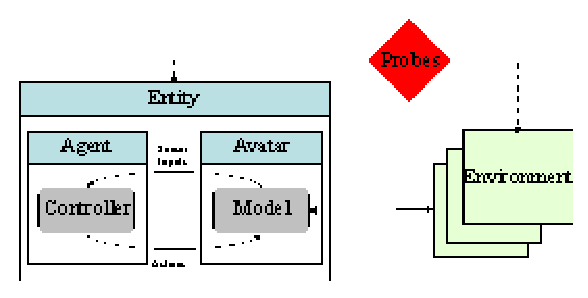
\includegraphics[width=\textwidth]{SweepDiagram}
	\caption
		[High-level overview of the \SWEEP{} architecture.]
		{High-level overview of the \SWEEP{} architecture showing the relationship between the major components.}
  \end{minipage}
\label{fig:SweepDiagram}
\end{figure}

\section{Simulation}
A SWEEP simulation is built from an XML simulation specification file. Within the specification file are six subsections, each defining a portion of the simulation. Using a pseudo-XML formatting, \refFigure{XMLconfig} lists and defines the six major subsections found in a SWEEP simulation specification.

Each XML subsection is passed to a \jclass{Builder}~\cite{GoF}, which may be explicitly specified, to parse its own section. The preferred parsing method is to recursively pass well-defined subsections to \jclass{Builder} objects that know how to handle that specific data. This design guideline is used throughout the implementation of \SWEEP{}. The \jclass{SimulationBuilder} receives the simulation section of the specification file, and then breaks that section into the six main sections. The \jclass{SimulationBuilder} then passes each subsection to the appropriate \jclass{Builder} associated with that section. This parsing strategy allows each section to define a custom syntax, which in turn provides for more flexible and usable component architectures by separating the data format from the data itself. For example, a \jclass{Controller} that uses a proprietary state machine library can use either an XML state machine encoding or a custom state machine encoding without requiring any modifications to the proprietary state machine code.

\begin{figure}[ht]
  \centering
  \begin{minipage}{5in}
    \centering
    \ttfamily
    \small
    \begin{tabbing}
      \hspace{4ex} \= \hspace{4ex} \= \kill
      $<$simulation$>$ \\
      \> $<$main$>$ \\
      \> \> \textnormal{Defines how the specified components should}    \\ 
      \> \> \textnormal{be connected together to create the simulation }\\
      \> $<$/main$>$ \\
      
      \> $<$agent$>$ \\
      \> \> \textnormal{Describes how the controller and the avatar interact,} \\
      \> \> \textnormal{defines state variables that will be needed} \\
      \> $<$/agent$>$ \\
      
      \> $<$controller $>$ \\
      \> \> \textnormal{Specifies the logic for an agent} \\
      \> $<$/controller$>$ \\
      
      \> $<$model$>$ \\
      \> \> \textnormal{Defines the platform to be simulated, used by the avatar} \\
      \> $<$/model$>$ \\
      
      \> $<$environment$>$ \\
      \> \> \textnormal{Setup of the context in which the agents interact} \\
      \> $<$/environment$>$ \\
      
      \> $<$probes$>$ \\
      \> \> \textnormal{Specification of data extraction and insertion} \\
      \> \> \textnormal{method, can be used for interactive GUIs} \\
      \> $<$/probes$>$ \\
      $<$/simulation$>$ \\
    \end{tabbing}
    \rmfamily
    \caption[A pseudo specification file for a \SWEEP{} simulation.]{Shown here is a pseudo specification file for a \SWEEP{} simulation.  The \SWEEP{} simulation specification defines six major subsections.  Each subsection defines characteristics for different aspects of the simulation.  The file uses an XML format.  \refAppendix{SweepSpecification} presents a complete \SWEEP{} XML specification file.}
    
  \end{minipage}
  
  \label{fig:XMLconfig}
\end{figure}

The default \jclass{Simulation} implements a sequential update strategy. First, the \jclass{Environment} is updated to ensure that any \jclass{Agent} decisions are based on current information. Then the \jclass{Entities} are updated by first updating the \jclass{Agent} that determines which \jclass{Actions} are to be performed by the \jclass{Avatar}. Then the \jclass{Avatar} is updated, executing commands from the \jclass{Agent}, resulting in an updated \jclass{State} for the next \jclass{Agent} update. Finally, any defined \jclass{Probes} are executed.  It is important to note that \SWEEP{} is not wedded to a sequential update strategy. Any update model, such as a fully threaded or a distributed  update model, can be implemented and used with \SWEEP{}.

\section{Agent}
An \jclass{Agent} has two main components, a \jclass{State} and a \jclass{Controller}. The \jclass{State} represents the current values of all variables that define the agent, and can be composed of both manifest and latent variables~\cite{jpolderman:SystemsTheoryBehavioral}.  A \italic{manifest variable} is something that the \jclass{Agent} has the ability to measure, whereas a \italic{latent variable} is only indirectly observable through the manifest variables (\eg, entropy).  Many of the manifest variables in a \jclass{State} object are values linked to \jclass{Sensors} in the \jclass{Environment}, thus providing a mechanism for cleanly communicating \jclass{Sensor} information from the \jclass{Environment} to the \jclass{Controller}.  Any latent variables are inferred by the \jclass{Agent} using information received directly from \jclass{Sensors}.

The \jclass{Controller} defines the logic by which the \jclass{Agent} is governed. Based on the current \jclass{State} of the \jclass{Agent}, the \jclass{Controller} determines what \jclass{Actions} should be executed by the \jclass{Avatar} associated with the \jclass{Agent}.  The default controller implemented for SWEEP is a finite state machine~\cite{plinz:FormalLanguages}. Finite state machines were chosen for their balance of power and simplicity.  A state machine uses sensor information from an \jclass{Avatar} as input, and \jclass{Actions} for the \jclass{Avatar} as output.  \refFigure{SimpleFSA} illustrates a trivial state machine that could be used by a \SWEEP{} \jclass{Agent}.  In the state machine, transitions are fired based on the state of three binary sensors.  When the sensors' states match a desired condition, the specified action is performed and the state machine moves to the next state.  For example, from state \texttt{s-1}, if all three sensors have a value of true (1), then the action \texttt{jmp} will be executed and the state machine will stay in state \texttt{s-1}.

In the simulation specification file, the state machine has two possible input formats: state-based and transition-based. In the state-based version, each state is defined by an XML section populated with the list of rules associated with that state.  In the transition-based version, the state machine section is populated by a list of transition rules that indicated the source state associated with the rules.  \refFigure{StateBasedFSA} and \refFigure{TransitionBasedFSA} show the state-based and transition-based formats of the state machine defined in \refFigure{SimpleFSA}.

\begin{figure}[ht]
  \centering
  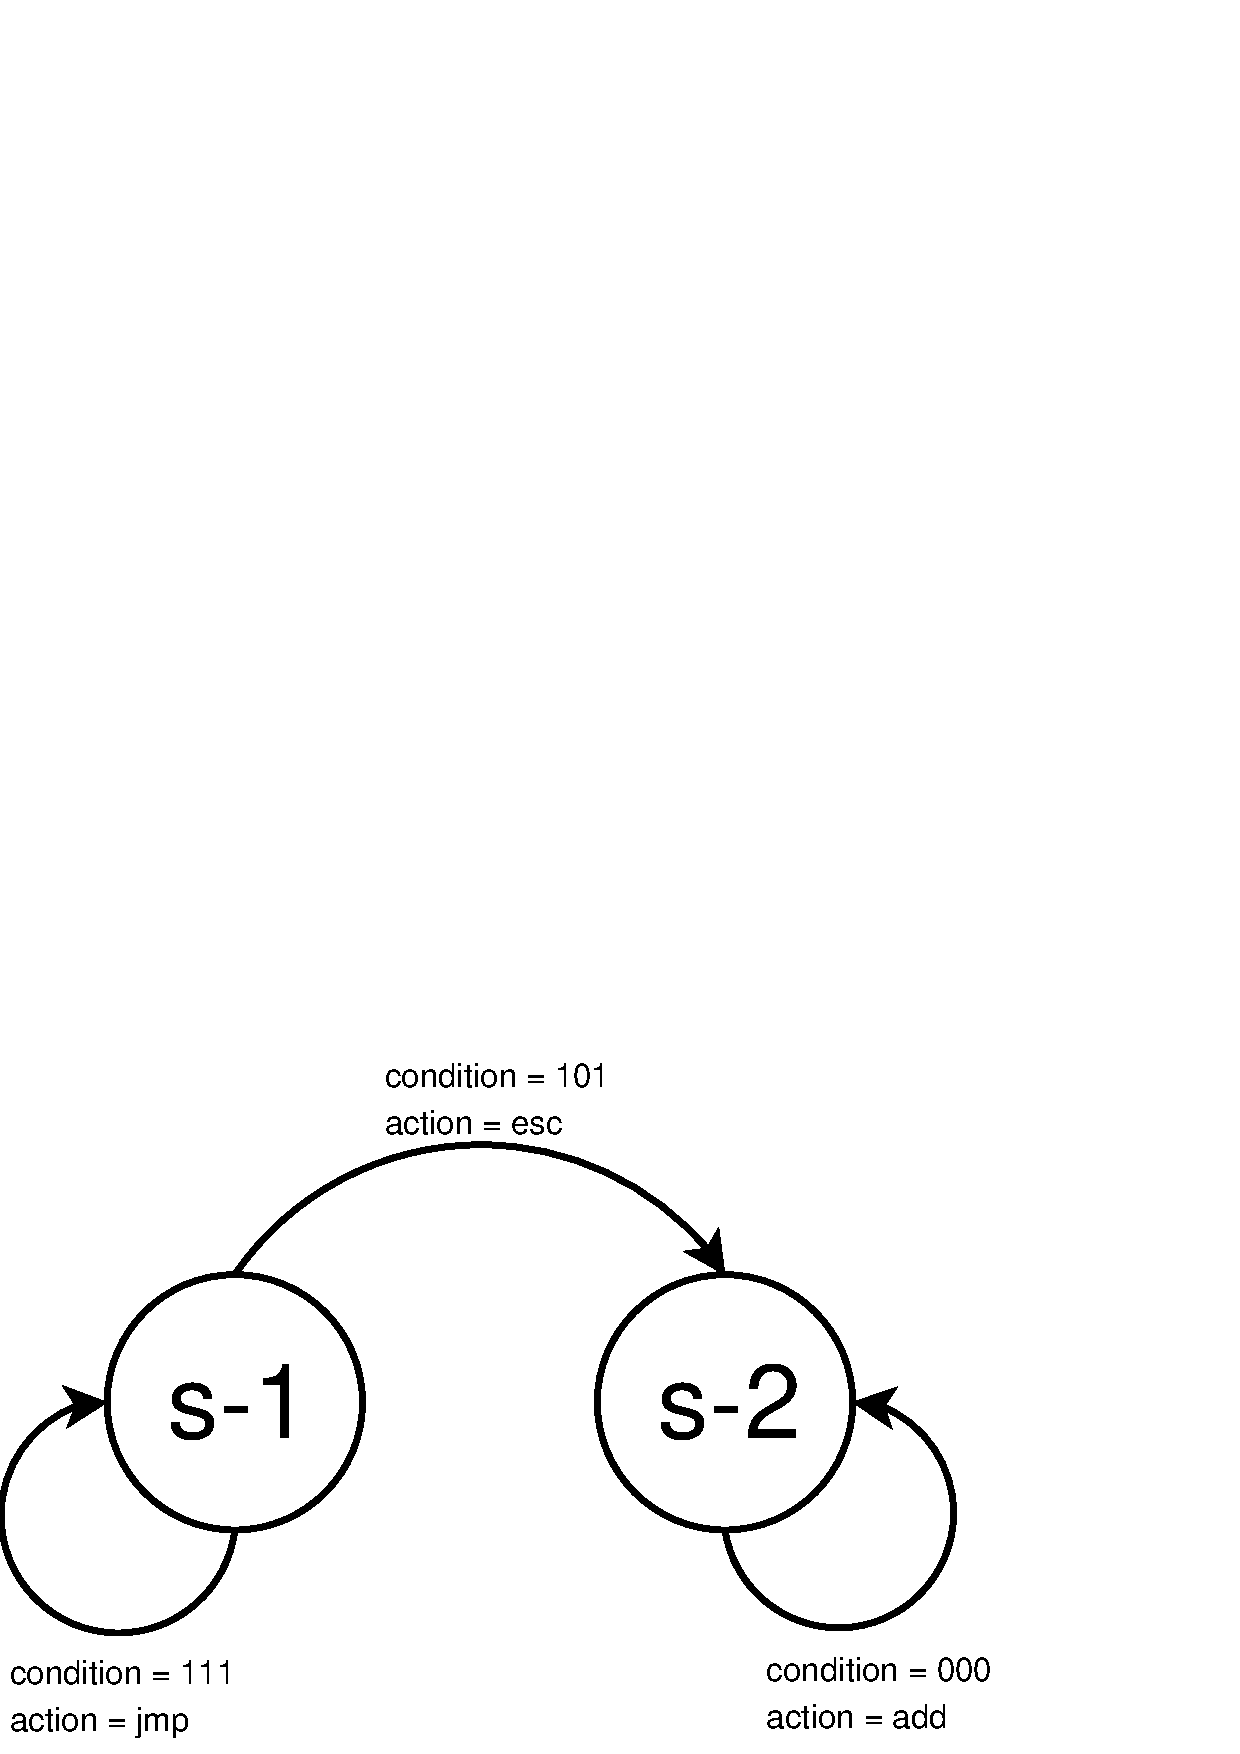
\includegraphics[scale=.5]{Figures/SimpleMachine.jpg}
\caption{A simple example of a finite state machine.}
\label{fig:SimpleFSA}
\end{figure}

\begin{figure}[ht]
  \singlespace
  \centering
  \fbox{
    \footnotesize
    \begin{minipage}{4.9in}
      \ttfamily
      <state name="s-1">\\
      ~~~<transition nextState="s-2" condition="101" action="esc"/>\\
      ~~~<transition nextState="s-1" condition="111" action="jmp"/>\\
      </state>\\
      <state name="s-2">\\
      ~~~<transition nextState="s-2" condition="000" action="add"/>\\
      </state>
    \end{minipage}
  }
\caption{State-based XML format of the finite state machine in \refFigure{SimpleFSA}.}
\label{fig:StateBasedFSA}
\end{figure}

\begin{figure}[ht]
  \singlespace{}
  \centering
  \fbox{
    \footnotesize
    \begin{minipage}{5.1in}
      \ttfamily
      <transition state="s-1" nextState="s-2" condition="101" action="esc"/>\\
      <transition state="s-1" nextState="s-1" condition="111" action="jmp"/>\\
      <transition state="s-2" nextState="s-2" condition="000" action="add"/>
    \end{minipage}
  }
\caption{Transition-based XML format of the finite state machine in \refFigure{SimpleFSA}.}
\label{fig:TransitionBasedFSA}
\end{figure}

\clearpage

\section{Avatar}
The \jclass{Avatar} is the part of the \jclass{Entity} that extends into the \jclass{Environment}. The purpose of the \jclass{Avatar} is two-fold. First, by separating the modeling of an \jclass{Agent} into an \jclass{Avatar}, it is easier to keep free the logic of the swarm algorithm from dependencies on environmental implementation issues. Secondly, the information abstraction ability of an \jclass{Avatar} allows an \jclass{Agent} to seamlessly interact with either a computer-model of the target platform, or an actual hardware platform whose sensors and actuators are networked into the simulation. This allows earlier hardware testing of swarm algorithms by mixing real and virtual platforms within the same scenario.

Every \jclass{Avatar} has an associated \jclass{Model} that dictates the characteristics and abilities of the platform being simulated. For example, a UAV model will dictate a minimum turning radius, maximum speed, and wing configuration. \jclass{Sensors} are the most important aspect defined by the \jclass{Model} because \jclass{Sensors} provide decision information to the \jclass{Agent}. The \jclass{Model} is also responsible for defining the \jclass{Actions} chosen by an \jclass{Agent}. Finally, the \jclass{Model} and the \jclass{Environment} are responsible for determining what, if any, direct methods of inter-agent communication are available.

\section{Environment}

The \jclass{Environment} defines the context in which the agents exist. The term \qw{environment} is used in a very broad manner in order to create the most flexible definition for the system. There are three core functionalities that the \jclass{Environment} is responsible for:

\begin{enumerate}
	\item Defining fundamental laws that \jclass{Avatar} objects must respect;
	\item Presenting an information abstraction layer for \jclass{Agent} interaction;
	\item Facilitating direct and indirect \jclass{Agent} interactions.
\end{enumerate}

Perhaps the most important functionality of the \jclass{Environment} is the role it plays as an information abstraction layer, which enables agents to \qw{sense} information about the environment without having to understand the implementation details of the environment. For example, the concept of a neighborhood is functionally different on a graph environment as opposed to a grid environment. However, to an agent whose ruleset depends on neighbor information, the meaning of the data does not need to change to accommodate different \jclass{Environment} implementations. Thus, the information abstraction component of the \jclass{Environment} object facilitates the creation of simulations where environments can be interchanged without a change to the logic of the agent.

Additionally,  the \jclass{Environment} is responsible for facilitating agent interactions. One of the key components of any swarm algorithm is the large number of both direct and indirect interactions between agents. Though some of these interactions may occur externally between different agents, the majority of interactions will take place within the context of the \jclass{Environment}, and thus will need to be mediated in order to minimize the need for agents to understand the implementation of the environment. For example, when an agent uses a pheromone to stigmergically communicate with other agents, an agent should not have to be concerned with how the chemical gradient information is stored and processed, just that it exists. Thus, facilitating agent interactions is a more specific way of presenting an agent-oriented information abstraction layer.

Finally, the \jclass{Environment} defines a set of rules or laws that must be adhered to by any \jclass{Avatar} associated with that particular \jclass{Environment}. Depending on the \jclass{Environment} implementation, these laws can range from constants (like gravity or the maximum network throughput) to constraints that must be satisfied or obeyed (\eg{} \textit{F=ma}, or no more that three agents can be resident on a node at any one time). It is through the definition and manipulation of these laws that environments with varying levels of complexity and fidelity can be constructed and interchanged.

\section{Probe}
The ability to interact with a running simulation through \jclass{Probes} is one of the most useful features of \SWEEP{}.  \jclass{Probes} in \SWEEP{} serve two purposes: to extract information from a simulation, and to insert information into a simulation. Possible uses for \jclass{Probes} include: generating animations of the simulation, storing statistical information on a simulation, or producing a user interface to allow a user to examine the effects of changing a parameter value during the execution of the simulation.

Due to the object models of modern programming languages, which restrict access to memory based on coarse permission models, completely unrestricted access to data for \jclass{Probes} is not entirely possible within the scope of a well-designed program.  A solution to this problem is the introduction of \jclass{Connectors} that serve as data conduits between components in \SWEEP{}.  The \jclass{Connector} concept is inspired by a number of design patterns, especially the \jclass{Proxy}~\cite{GoF} pattern and the \jclass{Listener} pattern as defined by Java~\cite{karnold:Java}.  

When a \jclass{Connector} is constructed, it is passed a reference to the two objects that it connects.  When one object wants to communicate with the other object, it actually invokes methods on the \jclass{Connector}.  The \jclass{Connector} then acts as a communications abstraction layer.  Any data passed through a \jclass{Connector} is made available to any \jclass{Probe}.  In a sense, \jclass{Probes} tap the communication lines in the same way one might tap a phone line.  Additionally, \jclass{Probes} are also able to delete or inject data into a \jclass{Connector}.  Thus, using \jclass{Connectors}, the full functionality of \jclass{Probes} is realized.  An example of how \jclass{Probes} might be used would be the construction of a diagnostic interface for a simulation.  The \jclass{Probes} provide the user interface with the current status of each \jclass{Agent} in the simulation, allowing the user to monitor the progress of each \jclass{Agent} individually or as a swarm.  Additionally, the user can direct changes in the environment, such as the availability of some resource, or even explicit changes in the behavior of single or multiple agents.
